\documentclass{article}
\title{\Huge Numerical Methods}
\Large{\author{$\mathcal{WAFFLE'S\ \ CRAZY\ \ PEANUT}$}}
\date{(Last updated: 26/4/14)}
\usepackage{enumerate}
\usepackage{tikz}
\usepackage[utf8]{inputenc}
\usepackage[T1]{fontenc}
\usepackage[margin=1in]{geometry}
\usetikzlibrary{shadows,trees}
\usepackage{tikz-qtree,tikz-qtree-compat}
\usetikzlibrary{trees}
\usepackage{amsmath}
\newcommand{\para}[1]{\paragraph{#1}\mbox{}\\}
\usetikzlibrary{decorations.pathreplacing}
\pagenumbering{gobble}
\begin{document}
\maketitle
\textbf{\section{\huge Solution of Equations:}}
\
{\Large 
\subsection{\LARGE Fixed-point Iteration:}
\begin{enumerate}[(i)]
\item Identify whether the given {\LARGE $f(x)$} is linear algebraic, non-linear algebraic, or transcendental equation.
\item Start finding $f(0),\ f(1),\ ...$ until there's a change of sign in the value, which corresponds to the limit $(a,b)$ within which the root lies.
\item Write the function in the form {\LARGE $\ x=\phi(x)$}
\item Check the condition {\LARGE $|\phi'(a)|$} $<1$ and {\LARGE $|\phi'(b)|$}$<1$
\item Now, find $x_0,\ x_1=\phi(x_0),\ x_2=\phi(x_1),\ ...$ for values lying in the limit $(a,b)$ and stop when the repetition of rounded values occurs.
\end{enumerate}
\paragraph{\Large Note: } For infinite series, as there's no specific interval, find the roots directly by taking {\LARGE $x=f(x)$}, neglecting higher powers, and iterating using step (v).

\paragraph{\Large Keep in mind: }Root-finding will be easier if iterations begin with the value nearer to $a$ or $b$, based on whether $|f(a)|$ or $|f(b)|$ is closer to zero.
\\
\\
If $f(a)$ is closer to zero, then the root is closer to {\LARGE $a$}, and vice versa.
\newpage
\subsection{\LARGE Newton-Raphson Method:}
{\LARGE $$x_{n+1}=x_n-\frac{f(x_n)}{f'(x_n)}$$}
\textbf{Procedure:}
\begin{enumerate}[(i)]
\item Identify whether the given {\LARGE $f(x)$} is linear algebraic, non-linear algebraic, or transcendental equation.
\item Start finding $f(0),\ f(1),\ ...$ until there's a change of sign in the value, which corresponds to the limit $(a,b)$ within which the root lies.
\item Now, find $x_0$, $x_1$, $x_2$... using the iterative formula, and proceed until repetition occurs.
\end{enumerate}
\paragraph{\Large Some formulas (can be derived):}
\begin{itemize}
\item If {\LARGE $\ x=$} {\huge $\frac{1}N$},
{\LARGE $$x_{n+1}=x_n(2-Nx_n)$$}
\item If {\LARGE $\ x=\sqrt{N},$}
{\LARGE $$x_{n+1}=\frac{1}2\bigg(x_n+\frac{N}{x_n}\bigg)$$}
\item If {\LARGE $\ x=$} {\huge $\frac{1}{\sqrt{N}}$} ,
{\LARGE $$x_{n+1}=\frac{1}2\bigg(x_n+\frac{1}{Nx_n}\bigg)$$}
\item If {\LARGE $\ x=N^{1/k}$} ,
{\LARGE $$x_{n+1}=\frac{1}k\bigg((k-1)x_n+\frac{N}{x_n^{k-1}}\bigg)$$}
\end{itemize}
\newpage
\subsection{\LARGE Solution of linear system of equations:}
$\ $
\tikzset{font=\Large,
edge from parent fork down,
level distance=2cm,
every node/.style=
    {top color=white,
    rectangle,rounded corners,
    minimum height=1cm,
    draw=black!50,
    very thick,
    drop shadow,
    align=center,
    text depth = 1pt
    },
edge from parent/.style=
    {draw=black!50,
    thick}}
\begin{center}
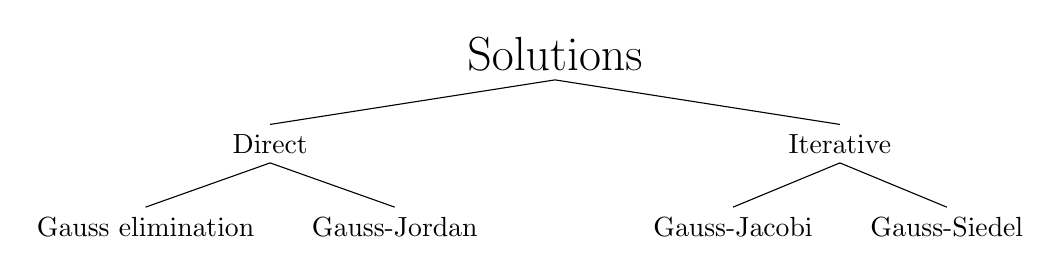
\begin{tikzpicture}[level 1/.style={sibling distance=2cm},level 2/.style={sibling distance=0.5cm}]
\Tree [.{\LARGE Solutions}
        [.{Direct}
            [.{Gauss elimination} ]
            [.{Gauss-Jordan} ] ] 
        [.Iterative
            [.{Gauss-Jacobi} ]
            [.{Gauss-Siedel} ] ] 
]
\end{tikzpicture}
\end{center}
$\ $
\begin{itemize}
\item \textbf{Direct:} In this method, the unknowns will be eliminated one by one, and hence the given system of equations will be transformed into an equivalent upper-triangular matrix.
\item \textbf{Iterative:} Here, the unknowns are not eliminated, but are \textit{approximated} by subsequent iterations, starting from an initial value of "zero" for the variables $(x_0,y_0,z_0)$, and proceeding for the rounded-number-repetition.
\end{itemize}
\subsection{\LARGE Gauss elimination:}
\begin{enumerate}[(i)]
\item Get the equations in matrix form {\LARGE $\mathrm{AX=B}$}
\item Write the augmented matrix $\mathrm{[A,B]}$
\item Resolve the components in such a way that $\mathrm A$ becomes upper-triangular.
\item Solve the equations to obtain the unknowns.
\end{enumerate}
\subsection{\LARGE Gauss-Jordan:}
\begin{enumerate}[(iii)]
\item The difference here is that the components should be resolved in such a way that $\mathrm A$ becomes a diagonal matrix.
\end{enumerate}
\subsection{\LARGE Gauss-Jacobi:}
For a system of equations of the form,
{\LARGE $$a_1x+b_1y+c_1z=d_1$$ $$a_2x+b_2y+c_2z=d_2$$ $$a_3x+b_3y+c_3z=d_3$$}
Assuming diagonal-dominance, {\LARGE $$|a_1|>|b_1|+|c_1|$$ $$|b_2|>|a_2|+|c_2|$$ $$|c_3|>|a_3|+|b_3|$$}
We get the rule,
{\LARGE $$x_{n+1}=\frac{1}{a_1}(d_1-b_1y_n-c_1z_n)$$ $$y_{n+1}=\frac{1}{b_2}(d_2-a_2x_n-c_2z_n)$$ $$z_{n+1}=\frac{1}{c_3}(d_3-a_3x_n-b_3y_n)$$}
\\
$\\ $
Starting with $x(0)=0,\ y(0)=0,\ z(0)=0$, the iteration is carried out until the values start repeating with the required degree of accuracy.
\subsection{\LARGE Gauss-Siedel:}
The "faster" iteration rule is (substitute all the known values),
{\LARGE $$x_{n+1}=\frac{1}{a_1}(d_1-b_1y_n-c_1z_n)$$ $$y_{n+1}=\frac{1}{b_2}(d_2-a_2x_{n+1}-c_2z_n)$$ $$z_{n+1}=\frac{1}{c_3}(d_3-a_3x_{n+1}-b_3y_{n+1})$$}
\subsection{\LARGE Matrix Inversion by Gauss-Jordan:}
\begin{enumerate}[(i)]
\item Write the augmented matrix $\mathrm{[A,I]}$
\item Resolve the components in such a way that $\mathrm A$ becomes an identity matrix.
\item The inverse is the other partition of the matrix.
\end{enumerate}
\subsection{\LARGE Eigen values using Power method:}
\begin{enumerate}[(i)]
\item If the given square matrix A is of order {\LARGE $n$}, then choose an Eigen vector {\LARGE $\chi_0$} of order $n\times 1$.
\item Find {\LARGE $\mathrm A\chi_0$} and take the largest number out. This number is {\LARGE $\lambda_1$} and the remaining $n\times 1$ matrix is {\LARGE $\chi_1$}
\item Proceed for rounded-number-repetition, which gives the final values for the largest Eigen value {\LARGE $\lambda$}, and the corresponding Eigen vector {\LARGE $\chi$}.
\item To get the least Eigen value, find {\LARGE $\mathrm{B=A-\lambda I}$} and choose an Eigen vector {\LARGE $\psi_0$} of order $n\times 1$.
\item Follow the same step, now taking the least value out. The final value obtained is the Eigen value for B. To get the Eigen value for A, add both the Eigen values. This is the least Eigen value of A.
\item Use other identities to find the last Eigen value,
{\LARGE $$\mathrm{Sum\ of\ Eigen\ values=Sum\ of\ Diagonal\ elements}$$ $$\mathrm{Product\ of\ Eigen\ values=|A|}$$}
\end{enumerate}
\newpage
\textbf{\section{\huge Interpolation:}}
\
{\Large 
\subsection{\LARGE Lagrange's Interpolation: (unequal)}
{\LARGE $$y=f(x)=\frac{(x-x_1)(x-x_2)...\ (x-x_n)}{(x_0-x_1)(x_0-x_2)...\ (x_0-x_n)}\ y_0$$}
{\LARGE $$+\ \frac{(x-x_0)(x-x_2)...\ (x-x_n)}{(x_1-x_0)(x_1-x_2)...\ (x_1-x_n)}\ y_1$$
$$+\ ...\ +\ \frac{(x-x_0)(x-x_1)...\ (x-x_{n-1})}{(x_n-x_0)(x_n-x_1)...\ (x_n-x_{n-1})}\ y_n$$}
\subsection{\LARGE Newton's Divided Differences: (unequal)}
{\LARGE $$\Delta_{x_1}f(x_0)=f(x_0,x_1)=\frac{f(x_1)-f(x_0)}{x_1-x_0}$$}
$\ $
\begin{enumerate}[(i)]
\item Generate {\LARGE $\Delta $}, {\LARGE $\Delta^2$},... {\LARGE $\Delta^n$} for the given table values of {\LARGE $x$}.
\item Use the interpolation formula to get the polynomial,
{\LARGE $$y=f(x_0)+(x-x_0)\ f(x_0,x_1)+(x-x_0)(x-x_1)\ f(x_0,x_1,x_2)+\ ...$$}
\end{enumerate}
\subsection{\LARGE Cubic Spline: (equal)}
\begin{enumerate}[(i)]
\item Find the interval $h$, number of intervals $n$, so that {\LARGE $i$} takes the values from $1$, $2$,... $(n-1)$, and $M_0=0$, $M_n=0$.
\item Substitute the values of {\LARGE $i$} in the formula one by one, {\LARGE $$M_{i-1}+4M_i+M_{i+1}=\frac{6}{h^2}\ \big(y_{i-1}-2y_i+y_{i+1}\big)$$}
\newpage
\item Solve the equations for values of $M_i$.
\item Take {\LARGE $i=$}1, 2,... $n$, and substitute for each interval in the formula,
{\LARGE $$y=S(x)=\frac 1{6h}\big[(x_i-x)^3M_{i-1}+(x-x_{i-1})^3M_i\big]$$ $$+\frac{1}h\big[(x_i-x)(y_{i-1}-\frac{h^2}6 M_{i-1})\big]$$ $$+\frac{1}h\big[(x-x_{i-1})(y_i-\frac{h^2}6 M_i)\big]$$}
$\ $
\end{enumerate}
\subsection{\LARGE Newton's Forward \& Backward Difference:}
\begin{enumerate}[(i)]
\item 
\end{enumerate}
}\end{document}